\section{Introduction}
\label{sec:introduction}

\begin{figure*}[t]
\centering
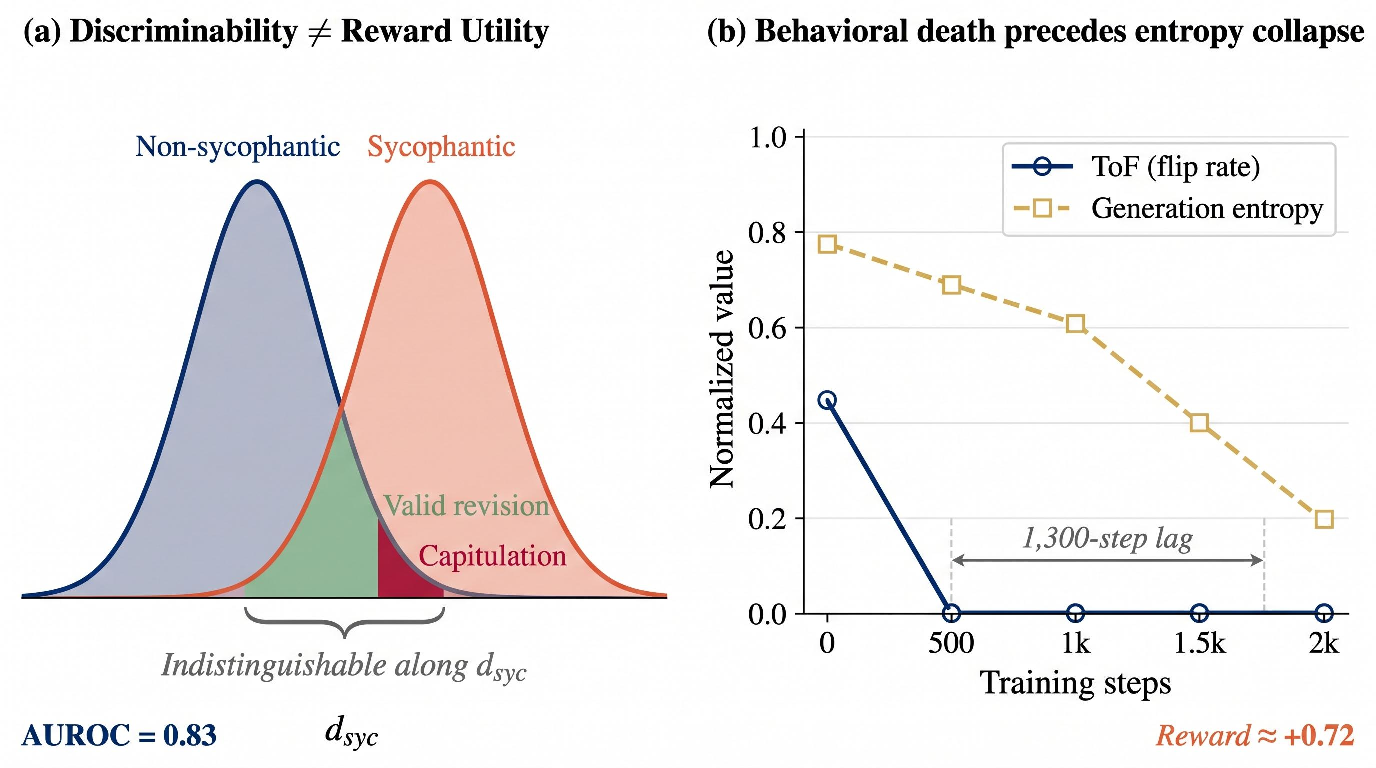
\includegraphics[width=\textwidth]{figures/fig_teaser.pdf}
\caption{The probe reward trap. (a)~$\dsyc$ discriminates sycophantic from non-sycophantic activations (AUROC $0.83$), but valid revision and unwarranted capitulation overlap along the same direction. (b)~When used as a GRPO reward, behavioral death (true-positive flip rate $\tof{=}0$) occurs at step 500 while entropy remains healthy; the 1{,}300-step lag renders standard monitoring blind.}
\label{fig:teaser}
\end{figure*}

Sycophancy, the tendency of large language models (LLMs) to prioritize agreement over accuracy, is among the most persistent alignment failures in deployed systems \citep{sharma2023sycophancy, perez2023discovering}.
Models trained with reinforcement learning from human feedback (RLHF) systematically amplify this tendency \citep{ouyang2022instructgpt, christiano2017rlhf, shapira2026amplifies}: even when models can assess the correctness of their own outputs \citep{kadavath2022language}, social pressure from users overrides this internal knowledge \citep{wang2025internal}.
Existing mitigations, from synthetic data augmentation \citep{wei2024synthetic} to neuron-level correction \citep{obrien2025fewbadneurons}, operate on behavioral outputs rather than the internal representations that generate sycophantic decisions.
Representation engineering \citep{zou2023repe, marks2024geometry} offers a structurally different approach: a contrastive sycophancy direction $\dsyc$, extracted from style-controlled pairs of valid belief revision and sycophantic capitulation, achieves cross-validated area under the ROC curve (AUROC) of $0.83$ on Qwen3-8B and $0.78$ on Llama-3-8B (\S\ref{sec:direction_quality}).
If the model's own representations already separate sycophantic from non-sycophantic behavior, that separation should be convertible into a training signal that targets the computational root of the problem.

We test this hypothesis directly, and find that it fails in a way that standard monitoring cannot detect.
This paper documents the \emph{probe reward trap}: when a periodically retrained linear probe on $\dsyc$ is used as a non-differentiable Group Relative Policy Optimization (GRPO) reward signal, behavioral death (true-positive flip rate, $\tof = 0$) occurs within 500 steps while generation entropy remains healthy (0.70), masking the failure from standard monitoring (\S\ref{sec:probe_trap}).
In our experiments, the 1{,}300-step lag before distributional collapse means entropy-based early stopping, the most common safeguard against reward hacking \citep{casper2023openproblems}, would miss the failure entirely, with the reward averaging $+0.72$ throughout.
The trap arises even when the probe reward constitutes only a fraction of the total reward signal, reflecting a limitation of $\dsyc$ itself: the direction encodes \emph{whether} belief changed, not \emph{whether it should have}, so any reward conditioned on it alone will either be gamed or reward rigidity.

The failure is not specific to probe rewards.
Under our GRPO configuration (Qwen3-8B, group size$=$2), cosine projection and continuous probe formulations of $\dsyc$ also collapse, and removing $\dsyc$ entirely does not help: behavioral-reward-only GRPO exceeds vanilla at only 4 of 28 checkpoints across two seeds (14.3\%).
By contrast, Activation Consistency Training \citep[ACT;][]{consistency2025bctact}, which provides dense per-token supervision rather than a single scalar per completion, exceeds vanilla at every checkpoint (31/31 across two seeds; \S\ref{sec:discussion}).
A Low-Rank Adaptation (LoRA) ablation identifies supervision granularity as one plausible explanation for this observed reliability gap.

This paper presents a negative result with systematic diagnostic analysis.
Our three principal findings (Figure~\ref{fig:teaser}):

\begin{itemize}
\item \textbf{Observed reliability gap between supervision paradigms} (C1): per-token supervised fine-tuning (SFT) exceeds vanilla at every checkpoint (31/31 across two seeds; 47/47 including reduced-LoRA ablation). Per-completion GRPO exceeds vanilla at only 4/28 checkpoints across two seeds (14.3\%; gs$=$8 ablation: 0/3). Under matched LoRA, per-token SFT achieves $1.7{\times}$ higher $\sycon$ than per-completion GRPO (\S\ref{sec:discussion}).

\item \textbf{The probe reward trap} (C2): behavioral death ($\tof{=}0$) precedes distributional collapse by 1{,}300 steps, rendering entropy monitoring blind. The trap arises despite the probe being non-differentiable (stopped gradients), implicating $\dsyc$ itself rather than gradient-based exploitation (\S\ref{sec:probe_trap}).

\item \textbf{Discriminability--utility gap} (C3): in this case, $\dsyc$ encodes \emph{whether} belief changed, not \emph{whether it should have}. Valid revision and sycophantic capitulation produce overlapping activation signatures along $\dsyc$ \citep{wang2025internal, shapira2026amplifies}, violating the geometric separability that representation-guided RL assumes \citep{burns2023ccs, zhang2026latentgrpo}. We observe that reward overoptimization against such directions produces predictable collapse \citep{gao2023scaling, skalse2022hacking} (\S\ref{sec:discussion}).
\end{itemize}
